% This .tex file (and associated .cls V2.5) produces:
%       1) The Permission Statement
%       2) The Conference (location) Info information
%       3) The Copyright Line with ACM data
%       4) NO page numbers
%
% as against the acm_proc_article-sp.cls file which
% DOES NOT produce 1) thru' 3) above.
%
% Using 'sig-alternate.cls' you have control, however, from within
% the source .tex file, over both the CopyrightYear
% (defaulted to 200X) and the ACM Copyright Data
% (defaulted to X-XXXXX-XX-X/XX/XX).
% e.g.
% \CopyrightYear{2007} will cause 2007 to appear in the copyright line.
% \crdata{0-12345-67-8/90/12} will cause 0-12345-67-8/90/12 to appear in the copyright line.
%
% ---------------------------------------------------------------------------------------------------------------
% This .tex source is an example which *does* use
% the .bib file (from which the .bbl file % is produced).
% REMEMBER HOWEVER: After having produced the .bbl file,
% and prior to final submission, you *NEED* to 'insert'
% your .bbl file into your source .tex file so as to provide
% ONE 'self-contained' source file.
%

\documentclass{sig-alternate-05-2015}
\usepackage{listings}
\usepackage{enumitem}
\usepackage{hyperref}
\usepackage{color,soul}

%\begin{comment}
\setlist[itemize]{noitemsep}
\setlist[description]{noitemsep}
%\end{comment}

% outcomment in final version 
\begin{comment}
\makeatletter
 \setcounter{page}{0}
\setcounter{tocdepth}{3}
\def\contentsname{Contents}
\def\tableofcontents{%
    \section*{\MakeUppercase{\contentsname}}%
    \@starttoc{toc}%
    }
\makeatother
\end{comment}

\begin{document}

\newcommand{\TITLE}{User Managed Virtual Clusters in Comet}

% Copyright
\CopyrightYear{2016} 
\setcopyright{acmcopyright}
\conferenceinfo{XSEDE16,}{July 17-21, 2016, , }
\isbn{978-1-4503-4755-6/16/07}\acmPrice{\$15.00}
\doi{http://dx.doi.org/10.1145/2949550.2949555}
%\setcopyright{acmcopyright}
%\setcopyright{acmlicensed}
%\setcopyright{rightsretained}
%\setcopyright{usgov}
%\setcopyright{usgovmixed}
%\setcopyright{cagov}
%\setcopyright{cagovmixed}


% DOI
%\doi{10.475/123_4}

% ISBN
%\isbn{123-4567-24-567/08/06}

%Conference
%\conferenceinfo{PLDI '13}{June 16--19, 2013, Seattle, WA, USA}

%\acmPrice{\$15.00}

%
% --- Author Metadata here ---
%\conferenceinfo{WOODSTOCK}{'97 El Paso, Texas USA}
%\CopyrightYear{2007} % Allows default copyright year (20XX) to be over-ridden - IF NEED BE.
%\crdata{0-12345-67-8/90/01}  % Allows default copyright data (0-89791-88-6/97/05) to be over-ridden - IF NEED BE.
% --- End of Author Metadata ---

\title{\TITLE}
%
% You need the command \numberofauthors to handle the 'placement
% and alignment' of the authors beneath the title.
%
% For aesthetic reasons, we recommend 'three authors at a time'
% i.e. three 'name/affiliation blocks' be placed beneath the title.
%
% NOTE: You are NOT restricted in how many 'rows' of
% "name/affiliations" may appear. We just ask that you restrict
% the number of 'columns' to three.
%
% Because of the available 'opening page real-estate'
% we ask you to refrain from putting more than six authors
% (two rows with three columns) beneath the article title.
% More than six makes the first-page appear very cluttered indeed.
%
% Use the \alignauthor commands to handle the names
% and affiliations for an 'aesthetic maximum' of six authors.
% Add names, affiliations, addresses for
% the seventh etc. author(s) as the argument for the
% \additionalauthors command.
% These 'additional authors' will be output/set for you
% without further effort on your part as the last section in
% the body of your article BEFORE References or any Appendices.

\numberofauthors{2}
\author{
% You can go ahead and credit any number of authors here,
% e.g. one 'row of three' or two rows (consisting of one row of three
% and a second row of one, two or three).
%
% The command \alignauthor (no curly braces needed) should
% precede each author name, affiliation/snail-mail address and
% e-mail address. Additionally, tag each line of
% affiliation/address with \affaddr, and tag the
% e-mail address with \email.
%
% 1st. author
\alignauthor
Rick Wagner, Philip Papadopoulos, Dmitry Mishin, Trevor Cooper, \\ 
Mahidhar Tatineti\\
       \affaddr{San Diego Supercomputer Center UCSD}\\
       \affaddr{9500 Gilman Drive \#0505}\\
       \affaddr{La Jolla, CA 92093-0505 USA}\\
       \email{rpwagner@sdsc.edu, phil@sdsc.edu, dmishin@sdsc.edu, tcooper@sdsc.edu}
\alignauthor
Gregor von Laszewski, \\
Fugang Wang, \\
Geoffrey C. Fox \\
       \affaddr{Indiana University}\\
       \affaddr{919 E. 10th Street}\\
       \affaddr{Bloomington, IN 47408}\\
       \email{laszewski@gmail.com, kevinwangfg@gmail.com}
}


\begin{comment}
\numberofauthors{7}
\alignauthor
Rick Wagner\\
       \affaddr{San Diego Supercomputer Center UCSD}\\
       \affaddr{9500 Gilman Drive \#0505}\\
       \affaddr{La Jolla, CA 92093-0505 USA}\\
       \email{rpwagner@sdsc.edu}
\alignauthor
Philip Papadopoulos\\
       \affaddr{San Diego Supercomputer Center UCSD}\\
       \affaddr{9500 Gilman Drive \#0505}\\
       \affaddr{La Jolla, CA 92093-0505 USA}\\
       \email{phil@sdsc.edu}
\alignauthor
Dmitry Mishin\\
       \affaddr{San Diego Supercomputer Center UCSD}\\
       \affaddr{9500 Gilman Drive \#0505}\\
       \affaddr{La Jolla, CA 92093-0505 USA}\\
       \email{dmishin@sdsc.edu}
\and
\alignauthor
Trevor Cooper\\
       \affaddr{San Diego Supercomputer Center UCSD}\\
       \affaddr{9500 Gilman Drive \#0505}\\
       \affaddr{La Jolla, CA 92093-0505 USA}\\
       \email{tcooper@sdsc.edu}
\alignauthor
Mahidhar Tatineti\\
       \affaddr{San Diego Supercomputer Center UCSD}\\
       \affaddr{9500 Gilman Drive \#0505}\\
       \affaddr{La Jolla, CA 92093-0505 USA}\\
       \email{mahidhar@sdsc.edu}
\alignauthor
Gregor von Laszewski\\
       \affaddr{Indiana University}\\
       \affaddr{919 E. 10th Street}\\
       \affaddr{Bloomington, IN 47408}\\
       \email{laszewski@gmail.com}
\and
\alignauthor
Fugang Wang\\
       \affaddr{Indiana University}\\
       \affaddr{919 E. 10th Street}\\
       \affaddr{Bloomington, IN 47408}\\
       \email{kevinwangfg@gmail.com}
}
\end{comment}

\begin{comment}
% out comment for final version
\begin{center}
{\Large \TITLE}
\end{center}
\tableofcontents

\newpage
\end{comment}

\maketitle

\begin{abstract}
Hardware virtualization has been gaining a significant share of computing time
in the last years. Using virtual machines (VMs) for parallel computing is an
attractive option for many users. A VM gives users a freedom of choosing an
operating system, software stack and security policies, leaving the physical
hardware, OS management, and billing to physical cluster administrators. The
well-known solutions for cloud computing, both commercial (Amazon Cloud, Google
Cloud, Yahoo Cloud, etc.) and open-source (OpenStack, Eucalyptus) provide
platforms for running a single VM or a group of VMs. With all the benefits,
there are also some drawbacks, which include reduced performance when running
code inside of a VM, increased complexity of cluster management, as well as the
need to learn new tools and protocols to manage the clusters.

At SDSC, we have created a novel framework and infrastructure by providing virtual
HPC clusters to projects using the NSF sponsored {\em Comet} supercomputer.
Managing virtual clusters on {\em Comet} is similar to managing a bare-metal 
cluster in terms of processes and tools that are employed. This is beneficial because
such processes and tools are familiar to cluster administrators. Unlike
platforms like AWS, {\em Comet}'s virtualization capability supports
installing VMs from ISOs (i.e., a CD-ROM or DVD image) or via an isolated
management VLAN (PXE). At the same time, we're helping projects take advantage
of VMs by providing an enhanced client tool for interaction with our management
system called Cloudmesh client. Cloudmesh client can also be used to manage
virtual machines on OpenStack, AWS, and Azure.

The article describes our design and approach to running virtual clusters, the
tools we developed, and initial user experience.
\end{abstract}

%
% The code below should be generated by the tool at
% http://dl.acm.org/ccs.cfm
% Please copy and paste the code instead of the example below. 
%
\begin{CCSXML}
<ccs2012>
<concept>
<concept_id>10010520.10010521.10010528</concept_id>
<concept_desc>Computer systems organization~Parallel architectures</concept_desc>
<concept_significance>500</concept_significance>
</concept>
<concept>
<concept_id>10011007.10010940.10010941.10010942.10010948</concept_id>
<concept_desc>Software and its engineering~Virtual machines</concept_desc>
<concept_significance>500</concept_significance>
</concept>
</ccs2012>
\end{CCSXML}

\ccsdesc[500]{Computer systems organization~Parallel architectures}
\ccsdesc[500]{Software and its engineering~Virtual machines}

%
% End generated code
%

%
%  Use this command to print the description
%
\printccsdesc

% We no longer use \terms command
%\terms{Theory}

\keywords{Virtual machine; Supercomputer;}

\newcommand{\Comet}{{\em Comet\/}}

\section{Introduction} \label{S:introduction}

The national cyberinfrastructure trends supported
by the National Science Foundation includes two important classes. The
first is the tradition support of large scale parallel computing needs
by sophisticated scientific applications and tightly coupled
high-performance computing clusters and supercomputers. The other is
the emerging long tail of computational science, driven by new
scientific domains (e.g., bioinformatics, computational sociology,
etc.) adopting the computer as a key tool for research and with
rapidly changing software environments and workflows suited to loosely
coupled systems, referred to as the ``long tail of
science'' \cite{comet14}. How to support these two classes of research
in an efficient manner is a challenge being faced at all scales:
departmental; campus; and nationally.

One approach to tackle this is to provide complete separate
machines and environments in support of both. However it is a valid
research question to ask whether the requirements for both classes could be provided by a joint
operational and hardware infrastructure. This is where \emph{Comet} \cite{comet14}
benefits the overall community by integrating some of
the requirements from both and providing a prototype which
combines these approaches. \emph{Comet's} goal is to primarily target
the long tail of science but its operation and use could be a model
for possible future systems.

In contrast to other systems providing virtualization capabilities,
\emph{Comet} does not deploy an IaaS framework such as OpenStack
\cite{openstack}. Instead, it is operated as a standard Linux cluster,
using a well known cluster management framework (Rocks
\cite{www-rocks}) and scheduler (Slurm \cite{slurm}) and integrates
virtualization concepts into them. As a result \emph{Comet}
uses the batch system to schedule, start, stop and manage VMs. This
obviously is of great advantage as on the same machine can provide a
traditional batch computing environment for established HPC users
while leveraging the benefits of a queuing system to dynamically
allocate physical resources for VMs. Moreover, the VMs have access to
the InfiniBand network using SR-IOV
\cite{sriov} and can perform RDMA operation between define groups of
VMs. This makes \emph{Comet} ideally targeted towards
hosting virtual clusters instead of just loosely coupled VMs.

We have ensured that the management of the virtual clusters (VC) allows
the use of common cluster tools such as Rocks, xCAT
\cite{www-xcat}, or Warewulf \cite{www-warewolf} using semantics based
off the experience of operating bare metal. This helps existing
cluster administrators quickly build and manage their VC by targeting
their current skills and tools. Once the VC is provisioned the
administrator can deploy a custom software environment supporting
their research group's unique needs. This is particularly valuable for
groups with rapidly evolving software stacks from an emerging
computational science field. Obviously such a model with integration
into the queuing system has the advantage of better
resource utilization in a resource starved environment but at the same
time provides the necessary performance benefits that advances
scientific applications need.

The paper is structured as follows. Next we provide some important
terminology that we use throughout the paper (Section
\ref{S:terminology}) and a more in depth look at  the motivation
(Section \ref{S:motivation}). We outline the architecture (Section
\ref{S:architecture}) and report on our client interface (Section
\ref{S:cloudmesh}). We present some preliminary results (Section
\ref{S:results}) and conclude our paper (Section \ref{S:conclusion}).


%!TEX root = virtual-clusters.tex

\subsection{Terminology}\label{S:terminology}

As the concept of using standard HPC infrastructure to manage virtual
clusters is new and introduces abstractions that may not be available
by standard virtualization frameworks such as OpenStack, AWS, and
Azure, we provide the necessary terminology that we will use
throughout this paper. The biggest difference we have is in the
introduction of computesets. The definitions include:

\begin{description}

\item[Node:] The term node is used to refer to individual computers in a virtual
cluster. The term node is synonymous with Virtual Machine (VM).

\item[Compute:] A node with substantial computational resources used to perform
work in a virtual cluster. Compute Nodes (CN) are started and stopped on request
by the cluster administrator.

\item[Frontend:] A node with limited computational resources used to manage a
virtual cluster. Frontend Nodes (FN) typically remain running 24 hours a day
and can be started and stopped on request by the cluster administrator

\item[Virtual cluster:] A virtual cluster (VC) is a loosely or tightly connected
network of FN and CNs managed together by a virtual cluster administrator.

\item[Computeset:] A group of CNs started together and being in some state
(submitted, started, finished, failed). Each CN can only belong to 1 {\em
computeset\/} in submitted or active state. Compute sets can be merged
to build a larger virtual cluster on demand.

\item[Image:] A file containing the contents and structure (ISO9660) of a disk
volume which can be attached as a cdrom to a node.

\item[Image attach:] Attach is an action applied to a node and image pair
whereby the contents of the image are made available to a node on the next power
on.

\item[Image detach:] Detach is an action applied to a node and image pair
whereby the contents of the image are made unavailable to the node on the next
power on.

\item[Console:] An interactive representation of the screen of a node (text or
graphical) provided to assist with node installation and management.

\end{description}


%!TEX root = virtual-clusters.tex

\subsection{Motivation} \label{S:motivation}

The reasons for creating the novel {\em Comet} virtual environment are
to define an efficient system architecture for virtual HPC clusters,
provide VC performance comparable to the underlying physical system,
and to deliver an HPC platfrom to the VC users and administrators in a
familiar fashion. VMs that are started on {\em Comet} are running on the same servers as regular
HPC jobs and VMs consequently have access to the same high-performance
hardware, including the InfiniBand interconnect via SR-IOV, local flash
drives, significant amounts of RAM and multicore CPUs with vector
instruction sets. Combined with the semantics and management
features we emphasize through our client interfaces we deliver near bare-metal
experience to the users and administrators of the VCs.  Hence the
abstraction of a virtual cluster mimics that of a physical one.

Two of the features that enable this bare-metal approach for
management are the private management VLAN and installation from an
ISO image. Each VC has its own VLAN, enabling the PXE-boot from a
frontend server and full control of an associated local network.  Via
this abstraction clusters can be management using existing tools
mentioned earlier, in addition to Cobbler \cite{cobbler} which also handles
bare-metal provisioning over a local network. Furthermore
we can leverage other commercial cluster management software as well,
like Bright Cluster Manager \cite{bright}.

For installation and troubleshooting, a VM can be booted up from a
regular ISO image uploaded to {\em Comet}'s
image server and mounted on the desired server on request. Using an
ISO is for many the easiest way to install a frontend of a cluster---a
machine running 24/7 and providing access and management for other
nodes. Users can also start a compute nodes using a regular ISO, or
PXE-boot from the frontend if an appropriate cluster management tool
has been set up. Hence compute nodes can be installed with minimum
effort while providing access to the desired OS supported by the KVM
hypervisor. There is no need to conduct complex manipulations of
images or limit use to a handful of sanctioned images. Users can
control the installation process by opening the {\em Comet} VM
console in a browser with the cloudmesh client tool (see Section \ref{S:cloudmesh}).

HPC admins have extensive experience working with bare-metal
clusters and the existing tools. Switching to new paradigms could require significant
resources in time, hardware and money spent to adopt such new
approaches. This also includes finding or writing new tools to adapt to
new system frameworks. {\em Comet}'s virtual environment makes running virtual
clusters straightforward by leveraging existing expertise of the
users. Using such well known tools will avoid the significant learning
curve associated for example with OpenStack as obvious from
\cite{ossurvey2016}.

The disk image management on {\em Comet} is a unique feature that
reduces the necessary storage and network infrastructure required
while also providing VMs with fast local storage. In short, the KVM
disk images for the VMs in a cluster are stored on a central server,
but migrated to the container while the VM is running and flushed back
when the VM is shut down. This lowers the effort needed for the
centralized storage server and limits the network bandwidth utilized
to transferring the image. This design also provides VMs with disk
performance based on the SSDs within the physical compute nodes.

In addition to production use of {\em Comet} VCs, the near bare-metal
approach makes {\em Comet} them an excellent platform for 
training. Groups can learn how to use tools that work on their real
systems in a controlled VM environment. With our solutions, we
demonstrate that VCs are 
easy to set up, replicate, reinstall, and destroy. A new
cluster can be booted up for a class and quickly torn down after its
intended use \cite{caida}. Hence, we provide an efficient platform for
trainees that need to get experience with software and services
supported by access which is very close to the real
hardware. Consequently, the huge benefit of our {\em Comet virtual
  clusters} is the combination of near bare-metal and VM features
while utilizing existing HPC batch systems.


%!TEX root = virtual-clusters.tex

\section{Architecture} \label{S:architecture}

We provide a brief overview of the system architecture and summarize
the components which support user managed virtual HPC clusters in {\em
  Comet}.

\begin{figure}[!h]
  %\centering
\vspace{-.5cm}
   \hspace{-1.5cm} 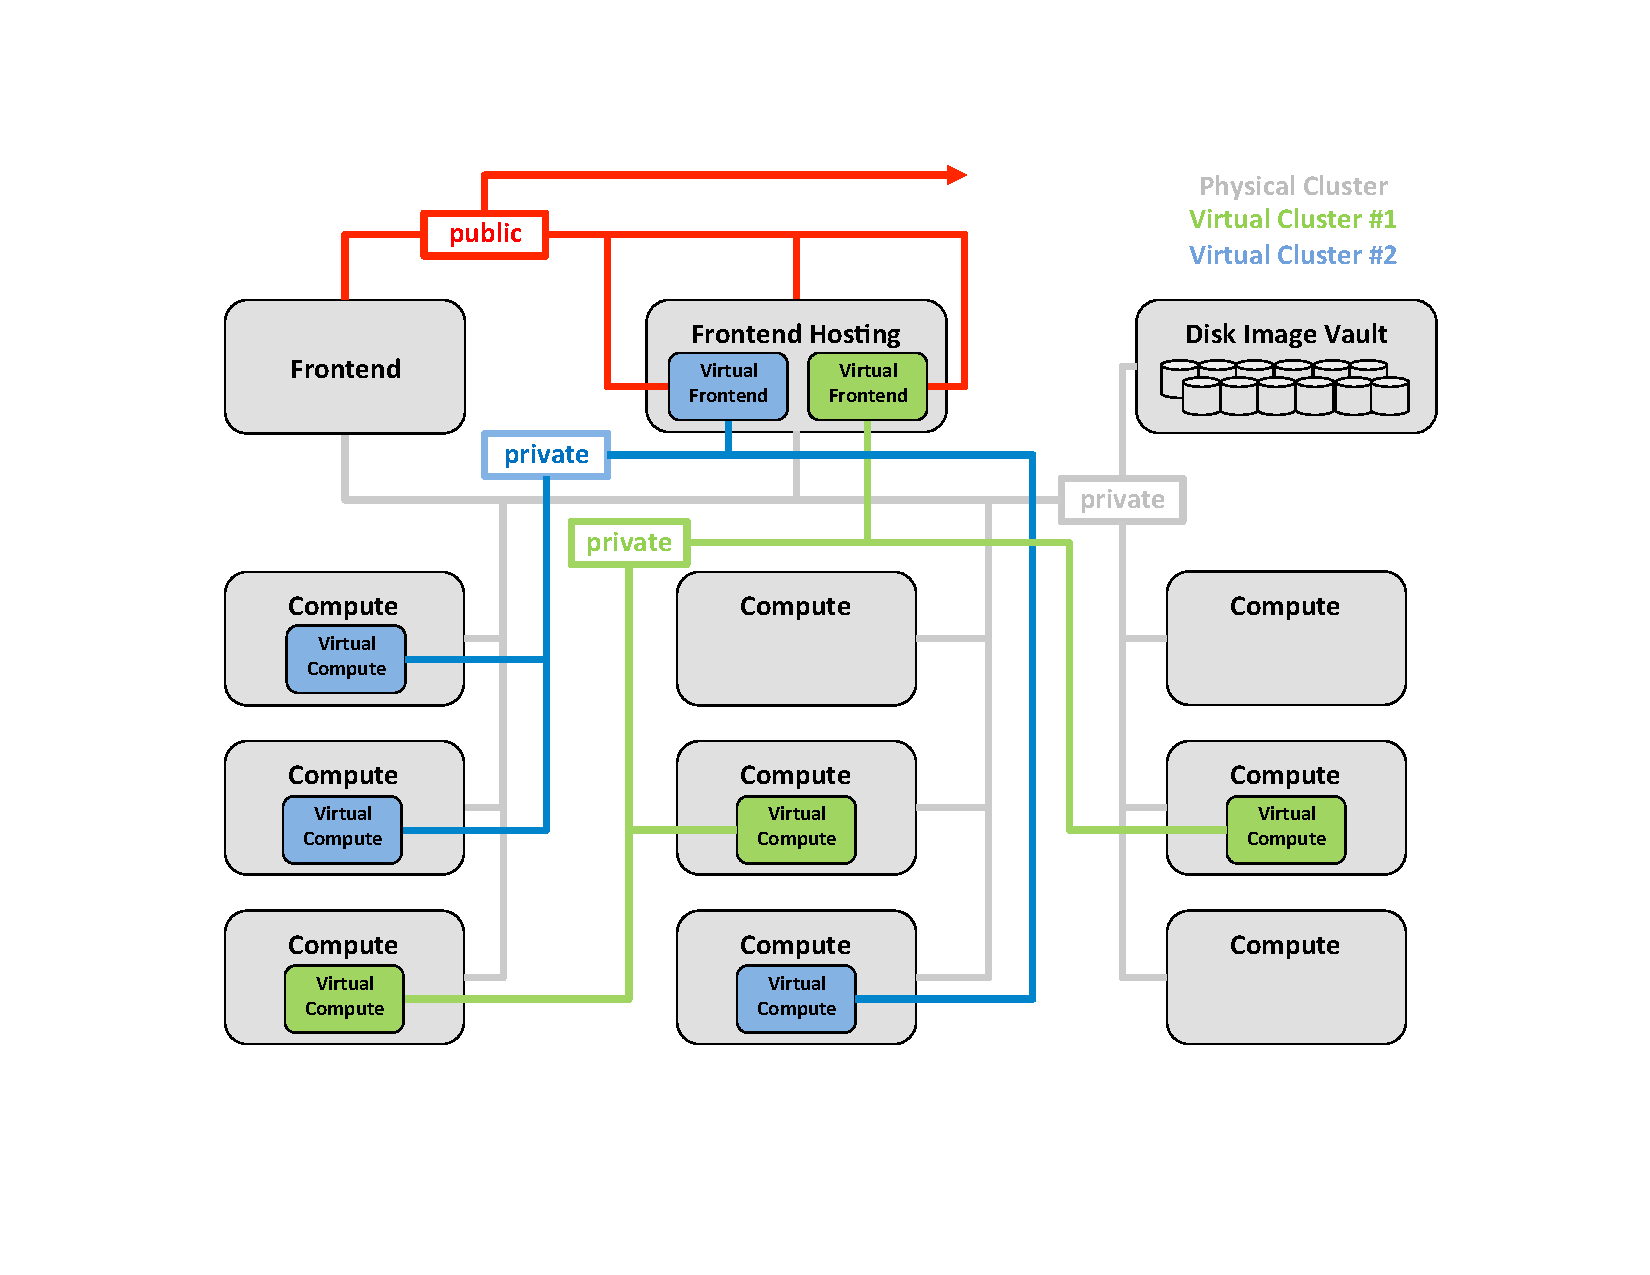
\includegraphics[width=1.3\columnwidth]{images/arch1}
\vspace{-1.5cm}

    \caption{Physical system architecture}
    \label{F:comet-arch1}
\end{figure}

{\parindent 0pt \bf Summary} The virtual cluster (VC) environment for {\em
Comet\/} is implemented largely on top of production HPC resources. {\em
Comet\/} standard compute nodes are used to host VC compute nodes (VCN) with
resource allocation managed by the production scheduler. The allocation of
standard compute nodes to the pool of nodes available for running VCNs can be
adjusted on demand.

Once a VC is defined on {\em Comet\/} a VC administrator is able to install the
VC frontend node (FN) with a system software management stack of their choice.
With the virtual FN installed and configured the VC administrator is able to start and
complete the installation and configuration of their VCNs. Installation of VCNs
can be interactive and manual or fully automated as all nodes can be PXE
installed inside the VC private network.

The resource usage of all VCNs is tracked as standard HPC jobs linked to
specific XSEDE allocations and usage is reported to XSEDE via the standard
mechanisms.

{\parindent 0pt \bf Nucleus.} The management platform we developed for this
coordination is called Nucleus and consists of a web service providing a REST API, a
database for maintaining state of managed resources, and a message queueing
system (based on RabbitMQ) providing connectivity and load balancing between
system components. Nucleus handles authentication and authorization of VC
administrators, tracks and orchestrates VCN state changes and resource
utilization, provides console access to the VC nodes using Guacamole
service. The state of VCNs is periodically pushed to the Nucleus management
database. The Nucleus database provides all needed information to VC
administrators requests for a state. The Nucleus database is ``eventually
consistent'' with the state of the physical cluster. This approach minimizes the
effect of VC administrator state requests on the production scheduler.

{\parindent 0pt \bf Rocks.} Rocks KVM roll provides the mechanism for running and
managing VMs on {\em Comet\/} physical hardware. Nucleus uses standard Rocks
commands to periodically query the state of all physical and virtual resources
and to execute commands on behalf of VC administrators to manage the resources
belonging to their VC.

\begin{figure}[!h]
  %\centering
\vspace{-.5cm}
     \hspace{-1.0cm} 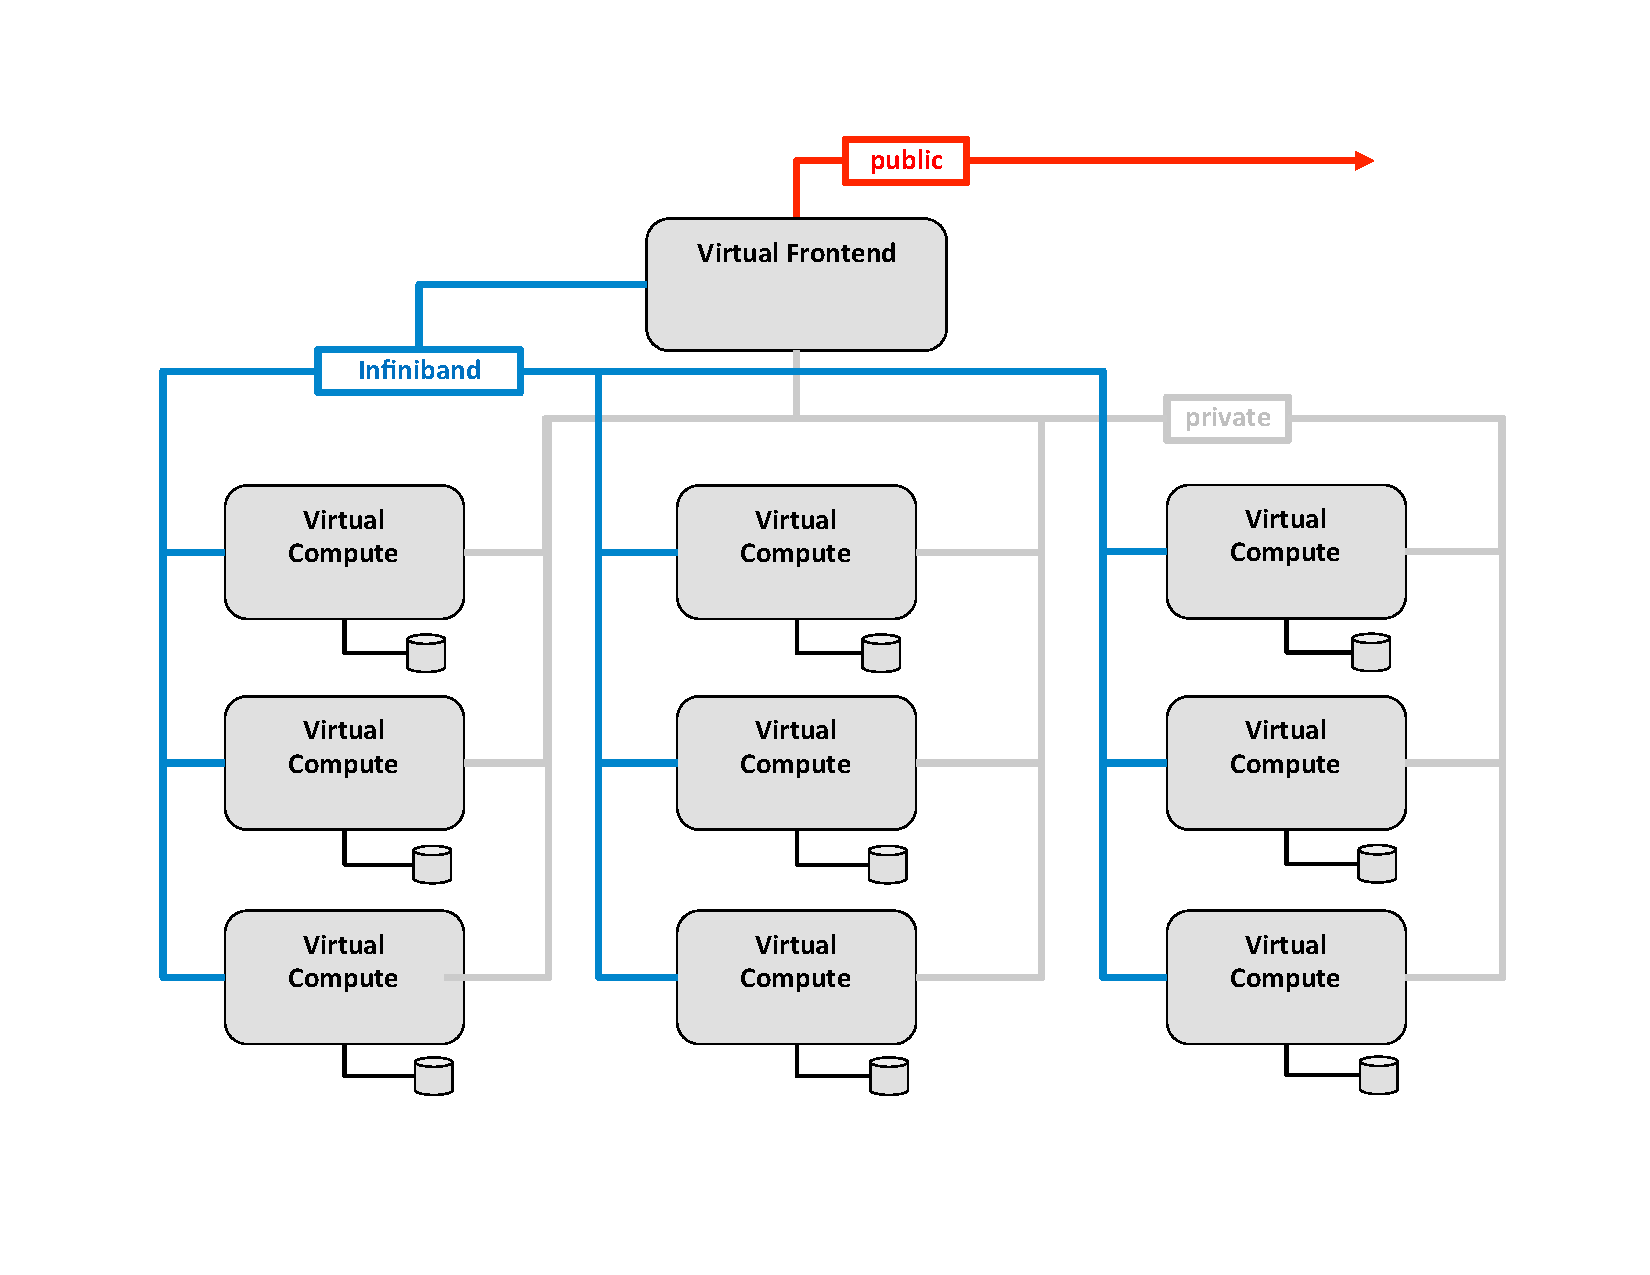
\includegraphics[width=1.2\columnwidth]{images/arch2}
\vspace{-1.5cm}
    \caption{Virtual cluster network topology}
\label{F:arch2}
\end{figure}

{\parindent 0pt \bf Networking.} Frontend and compute nodes are hosted on
physical hosts with two (private and public) or one (private) 10Gbps Ethernet
interfaces, respectively. The private network interfaces of all VMs in a VC are
connected to a logical VLAN device. Logical VLAN devices are raw, tagged packet
interfaces, using the Macvtap driver. Frontend public interfaces are bridged
either directly to a 10GbE interface or to a virtual VLAN device on the physical
host. Physical hosts also provide one FDR InfiniBand interface with one or more
Single Root IO Virtualization (SR-IOV) virtual functions enabled. All VMs of a
single VC are configured to use InfiniBand SR-IOV virtual functions with a
single common pkey.

{\parindent 0pt \bf Scheduling.} Frontend nodes run constantly at no charge and
provide access to the compute nodes of their associated virtual cluster. VC
administrators can start compute nodes on any physical compute node assigned by
the {\em Comet\/} scheduler.


%%% Local Variables:
%%% mode: latex
%%% TeX-master: t
%%% End:



\newcommand{\GET}{GET}
\newcommand{\DELETE}{DELETE}
\newcommand{\PUT}{PUT}
\newcommand{\POST}{POST}
\newcommand{\PATCH}{PATCH}


\begin{table*}[!h]
\caption{REST interface of the {\em Comet\/} virtual cluster service.}\label{T:rest}
\smallskip

\begin{small}
\begin{tabular}{|llp{6.5cm}|}
\hline
	& REST URL & Description \\
\hline
\GET	  & /v1/cluster/								     & gets the list of all clusters \\
\hline
\GET 	  & /v1/cluster/\{cluster.name\} 						     & Obtain details about the named cluster \\
\hline
\DELETE   & /v1/cluster/\{cluster.name\} 						     & Destroy the named cluster \\
\hline
\GET 	  & /v1/cluster/\{cluster.name\}/compute/\{compute.name\}		     & Obtain the details of a named compute resource  in a named cluster \\
\hline
\DELETE   & /v1/cluster/\{cluster.name\}/compute/\{compute.name\} 	      	     & Destroy the named compute resource in a  named cluster \\
\hline
\PUT 	  & /v1/cluster/\{cluster.name\}/compute/\{compute.name\}/attach        & iso Attach an ISO to the named compute resource in a named cluster   \\
\hline
\PUT 	  & /v1/cluster/\{cluster.name\}/compute/\{compute.name\}/poweroff      & Power off the named compute resource  in a named cluster \\
\hline
\PUT 	  & /v1/cluster/\{cluster.name\}/compute/\{compute.name\}/poweron 	     & Power on the named compute resource  in a named cluster \\
\hline
\PUT 	  & /v1/cluster/\{cluster.name\}/compute/\{compute.name\}/reboot 	     & Reboot the named compute resource in a  named cluster \\
\hline
\POST 	  & /v1/cluster/\{cluster.name\}/compute/\{compute.name\}/rename 	     & Rename the named compute resource  in a named cluster \\
\hline
\PUT 	  & /v1/cluster/\{cluster.name\}/compute/\{compute.name\}/reset 	     & Reset the named compute resource in a  named cluster \\
\hline
\PUT 	  & /v1/cluster/\{cluster.name\}/compute/\{compute.name\}/shutdown      & Shutdown the named compute resource in a named cluster  \\
\hline
\GET 	  & /v1/cluster/\{cluster.name\}/frontend/ 	     			     & Obtain the details of a frontend resource in a named cluster  \\
\hline
\PUT 	  & /v1/cluster/\{cluster.name\}/frontend/attach iso 			     & Attach an ISO to the frontendresource in a named cluster  \\
\hline
\PUT 	  & /v1/cluster/\{cluster.name\}/frontend/poweroff 		             & Power off the frontend of a named cluster  \\
\hline
\PUT 	  & /v1/cluster/\{cluster.name\}/frontend/poweron 			     & Power on the frontend of a named cluster  \\
\hline
\PUT 	  & /v1/cluster/\{cluster.name\}/frontend/reboot 			     & Reboot the frontend of a named cluster  \\
\hline
\PUT 	  & /v1/cluster/\{cluster.name\}/frontend/reset			     & Reset the frontend of a named cluster  \\
\hline
\PUT	  & /v1/cluster/\{cluster.name\}/frontend/shutdown 			     & Shutdown the frontend of a named cluster  \\
\hline
\GET 	  & /v1/cluster/\{cluster.name\}/compute/\{compute.name\}/console/  & Open VNC console to named  compute resource \\
\hline
\GET 	  & /v1/cluster/\{cluster.name\}/frontend/console/    	      		     & Open VNC console to name frontend resource  \\
\hline
\POST 	  & /v1/computeset/	  	  						     & Power on a set of computes creating a ComputeSet \\
\hline
\GET 	  & /v1/computeset/  								     & list the compute set \\
\hline
\GET 	   & /v1/computeset/\{computeset.id\} 						     & Obtain the details of the identified ComputeSet  \\
\hline
\PUT 	   & /v1/computeset/\{computeset.id\}/poweroff 					     & Power off the identified ComputeSet  \\
\hline
\PUT 	   & /v1/computeset/\{computeset.id\}/reboot					     & Reboot the nodes in the identified ComputeSet  \\
\hline
\PUT 	   & /v1/computeset/\{computeset.id\}/reset					     & Reset the nodes in the identified ComputeSet  \\
\hline
\PUT 	   & /v1/computeset/\{computeset.id\}/shutdown 					     & Shutdown the nodes in the identified ComputeSet  \\
\hline
\GET 	   & /v1/user 									     & Returns Users details in JSON format  \\
\hline
\PUT 	   & /v1/user 									     & Returns Users details in JSON format  \\
\hline
\PATCH 	   & /v1/user 									     & Returns Users details in JSON format  \\
\hline
\GET 	   & /v1/project 								     & Returns project details  \\
\hline
\GET 	   & /v1/image 								     & Gets the list of images  \\
\hline
\POST 	   & /v1/image 									     & Adds and image  \\
\hline
\end{tabular}
\end{small}


\end{table*}


{\parindent 0pt \bf Image Storage.} The implemtation of VCs in {\em Comet\/} also
requires a Network Attached Storage (NAS) (Disk Image Vault, Figure
\ref{F:comet-arch1}) --- a server with a large disk pool for VM images and ISO
files. VM images are stored as ZFS datasets on the NAS with each VM owning a
single image. The Image Storage system orchestrates the creation and destruction
of iSCSI targets providing read-only access to VM images resident on the NAS.
This allows VMs to start booting almost instantly. Image Storage also migrates a
copy of the VM image to the physical node hosting the VM and creates a local
temp-write volume to receive writes from the VM while the migration is underway.
After migration is complete the VM is briefly paused, the migrated VM image and
temp-write image are merged, the iSCSI target is disconnected and the VM is
resumed with both reads and writes accessing the local copy of the VM image.
At this point the VM is fully autonomous from the NAS providing great
capabilities of scaling without putting load on the NAS or network. Periodic
snapshots of the local, ZFS backed, VM images are automatically created and
copied back to the NAS keeping VM images backed up in case the physical node
crashes. The final synchronization of changes to VM images after VM shutdown
allows the VM image state to be persisted until the next VM boot.



{\parindent 0pt \bf Messaging.} We implemented an asynchronous communication
system between the components of the image management system, and also Nucleus
components connections using the AMQP messaging system RabbitMQ. We have Celery
workers running in several locations in the system, receiving AMQP messages with
jobs and normally replying with AMQP messages as well. This ensures smooth
operation under high loads by scheduling jobs in a queue rather than trying to
perform those as they come, and ease of scaling by adding more resources with
running daemons.

{\parindent 0pt \bf REST Interface}
In order to support the concept of virtual clusters on {\em Comet\/} we
provide a secure REST service to access them. The basic REST
signatures are listed in Table \ref{T:rest}. However the client
interface that uses these rest calls provide additional functionality
and allow easy scripting which is demanded by VC
administrators. We describe the client in Section \ref{S:cloudmesh}.



%!TEX root = virtual-clusters.tex
%%% Local Variables:
%%% mode: latex
%%% TeX-master: t
%%% End:

\section{Cloudmesh Client} \label{S:cloudmesh}

The Cloudmesh Client toolkit \cite{www-cloudmesh} is a lightweight
client interface for accessing heterogeneous clouds, clusters, and
workstations right from the user's computer.  The client has its
origin in \cite{Laszewski2007,laszewski09,laszewski10}. With the
client a user can manage their own set of resources enabling management of a
personalized cyber infrastructure. It includes an API, a commandline
client, and a commandline shell.  Extensibility is provided via
convenient abstractions.  A local database allows caching of
information from remote resources.  This is an essential feature of
Cloudmesh as it allows users to preserve a view of the infrastructure
even in cases where it may not be reachable. Obviously, such a cache is
especially useful for large scientific workflows and services that
require the management of many tasks.  Administrators naturally need
such a cached view in order to identify faults and to effectively
preserve the view of resources that need to be accessed or have been
created in the past.

Furthermore, users can, via the provided abstractions, switch easily
between or utilize together virtual machines from OpenStack, Amazon,
Azure Clouds, and \Comet~virtual clusters \cite{comet14}. Hence a greater ability to
deal with faults or system failures can be achieved. Cloudmesh Client
can be installed on Linux, OSX, and Windows. Currently we support
backends to SLURM, SSH, OpenStack, Azure, and AWS. A Docker interface
is planned.\footnote{In the past we supported AWS and Azure which we
  are integrating back into the client and will be available at time
  of publication. Our main focus so far was the ability to add
  OpenStack in support of upcoming systems such as Jetstream and
  virtual clusters such as used in \Comet } Next we provide a short
overview of the main features of the Cloudmesh Client.

{\parindent 0pt \bf Client based.} Cloudmesh Client as the name
indicates is a client based toolkit that installs and runs on the
users or administrators computers. An optional prototype portal is
also available as an add on.

{\parindent 0pt \bf Layered Architecture.} Cloudmesh Client has a
layered architecture (Figure \ref{F:arch-layer}) that allows easy
development of new features. This also allows contribution by the
community while developing integrated and smaller sub components. A
resource abstraction layer allows the integration of a multitude of
resources spanning HPC, Containers, and Cloud resources. This layered
architecture is augmented with a number of components (Figure
\ref{F:arch-component}) that together build the overall and expandable
Cloudmesh Client architecture providing a rich feature set.

\begin{figure}[!h]
  %\centering   
    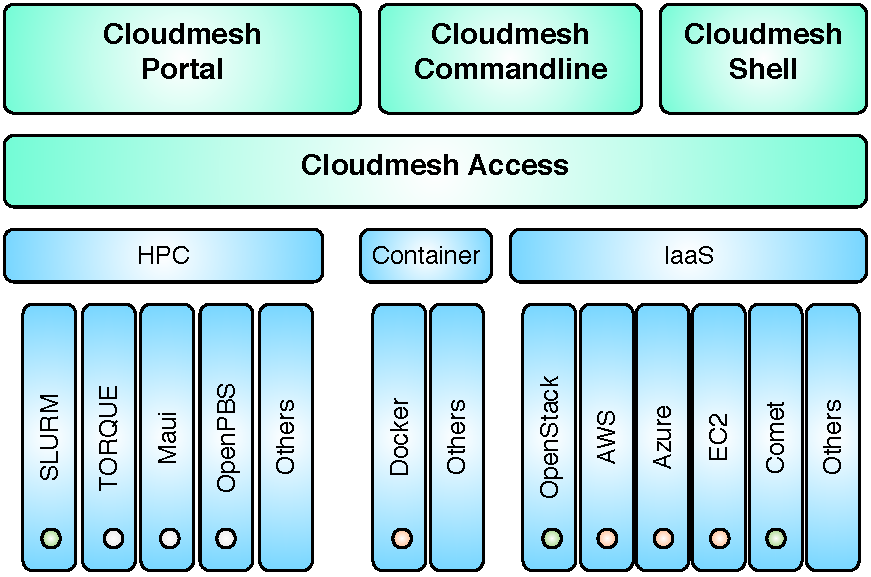
\includegraphics[width=1.0\columnwidth]{images/client/cloudmesh-arch-1.pdf}
    \caption{Cloudmesh layered architecture.}
    \label{F:arch-layer}
%\end{figure}
\bigskip
%\begin{figure}[!h]
  %\centering
    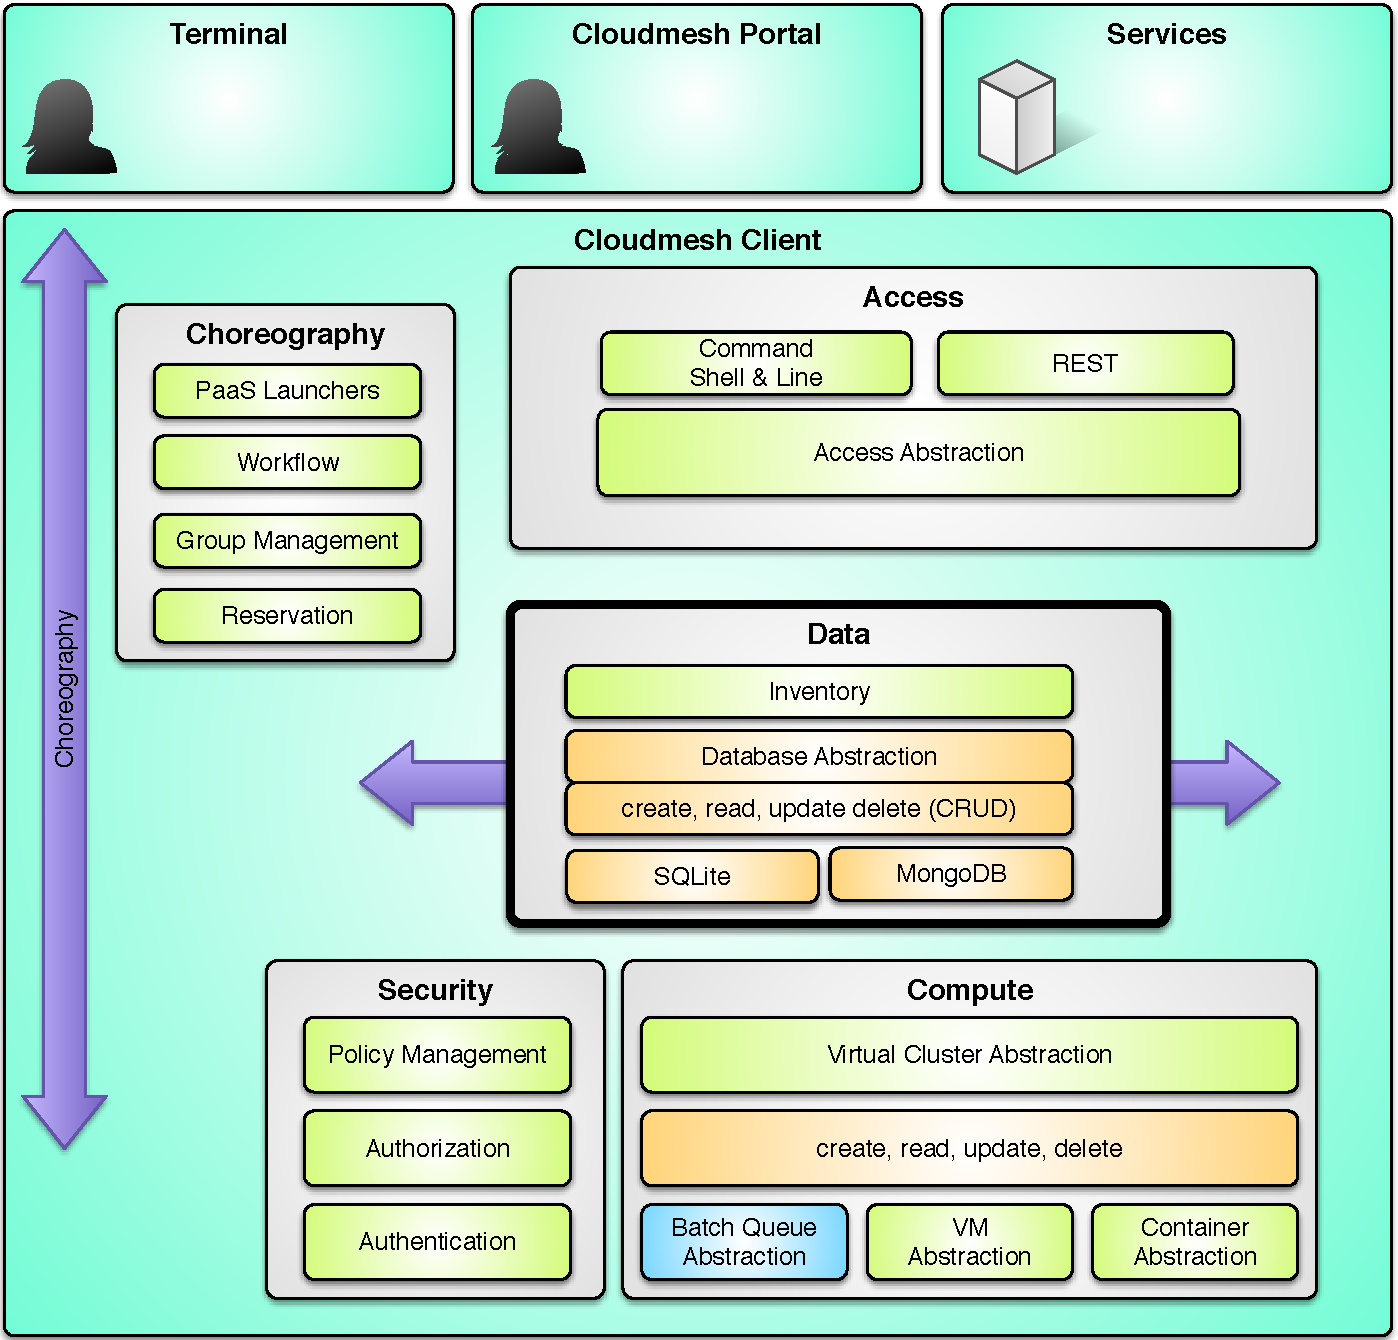
\includegraphics[width=1.0\columnwidth]{images/client/cloudmesh-arch-2.pdf}
    \caption{Cloudmesh component overview}
    \label{F:arch-component}
%\end{figure}

\bigskip

%\begin{figure}[htb]

{\tt cm comet cluster  ID}\newline -- Show the cluster details

{\tt cm comet start ID vm-ID-[0-3] --walltime=6h}\newline -- Boot 3 nodes for 6 hours

{\tt cm comet iso attach image.iso ID vm-ID-3}\newline -- Attach an iso image

{\tt cm comet power on ID vm-ID-0}\newline -- Power on node 0

{\tt cm comet console ID vm-ID-0}\newline
-- open the console for the node

\caption{Example Comet client commands}
\label{F:commands}
\end{figure}


\parindent 0pt { \bf State Caching.} Cloudmesh contains necessary state
about the resource and environment that a user may want to use.  The
information is managed in a database abstraction that would allow
storing the data in a variety of databases such as SQL and MongoDB. At
this time we have chosen SQLite to be the default database as it does
not require any additional setup and is universally available on all
operating systems without change. Previously we also provided a
MongoDB based backend system, but for the \Comet~client it is
beneficial to interact with the system without the need of additional
services.

{\parindent 0pt \bf Security Management.} For \Comet~users, it is
beneficial that access to the backend services are enabled with secure
credentials managed on the user's machine as well as with token based
service access.  This reflects best practice by many supercomputing
centers. Through abstractions integration with hosted security
services \cite{BasneyHW05} would also be possible.  However our
integration in clouds is naturally done outside such frameworks and
allows user to individually add their credentials for services such as
Azure, AWS, and other public clouds into the client easily. We have an
exploratory project in place that looks at the use of Yubikeys for
Cloudmesh Client and Cloudmesh Portal \cite{yubikey}. This will allow
an additional 2 factor authentication as part of accessing services
used by the users.  Hence, the Cloudmesh Client deals with the secured
connection and interaction by considering the appropriate interactions
with the different backends.  For the \Comet~virtualized cluster, it
handles the initial apikey retrieval, once a user is authenticated to
the nucleus service. It also handles all the subsequent calls in a
secured fashion by dealing with the messages signing, encryption and
decryption via utilizing proper libraries.

\parindent 0pt { \bf Command Shell and Command Line.} Cloudmesh contains a
command shell allowing scripts and interactive use. However we
designed the command shell in such a way that each command can also be
called from the command line reducing development and maintenance
efforts. Through the Cloudmesh database abstraction the state is
synchronized between different components.

\parindent 0pt { \bf Cloudmesh Client Portal.} Previously, we
distributed Cloudmesh with client, server, and a portal in one
package. This however turned out to be too complex to be installed for
some of our less technically skilled user communities. Thus we split up
the original Cloudmesh into multiple independent packages, such as the
{\em Cloudmesh Client} and the {\em Cloudmesh Portal}. The portal
provides currently a minimal feature set to manage virtual machines
and HPC jobs. It showcases how to integrate the client and the rest
services in more elaborated portal frameworks. We will expand upon the
existing features and make the portal more feature complete. Due to
our focus on the \Comet~community, the commandline client has an
increased development priority as it allows users to automatize
advanced {\em DevOps} workflows through scripting.

\parindent 0pt { \bf Cloudmesh Comet.} We are actively developing the
client interface for SDSC's \Comet~\cite{www-comet-user-manual}
supercomputer allowing near bare metal provisioning. The interface
reuses Cloudmesh components and technologies while interfacing with
the {\em Comet} Nucleus REST interface. Through this interplay the virtual
cluster administrators are enabled to utilize tools and services that
the they typically use to manage an on-premise bare metal cluster. As
part of this development we have developed an easy to use high level
command line interface specifically targeted to {\em Comet's\/} features. This
includes the following functionality:

\begin{itemize}
\item Configuring the nucleus service endpoint and the authentication
  tokens or keys.
\item Getting information and status of the users cluster(s), nodes,
  computesets, and other entities.
\item Power management of the cluster frontend node.
\item Request resource allocation to boot the users node(s); and release
  the resource upon completion.
\item Power management to shutoff, power on, reboot compute node(s)
  during the lifetime of the requested resource allocation.
\item Getting console access to the frontend node or a running compute
  node
\item System ISO image management. This includes listing available ISO
  images, upload new images, and attach/detach an ISO to/from one or
  more compute nodes.
\item Convenient management commands to, for example, renaming compute
  nodes either individually or in batch.
\end{itemize}

Some example commands are depicted in Figure \ref{F:commands}. The
manual page is shown in Figure \ref{F:man}.


%%% Local Variables:
%%% mode: latex
%%% TeX-master: t
%%% End:
\begin{figure}[!h]
\begin{small}
\begin{verbatim}
comet init
comet ll [CLUSTERID] [--format=FORMAT]
comet cluster [CLUSTERID][--format=FORMAT]
comet computeset [COMPUTESETID]
                 [--allocation=ALLOCATION]
                 [--cluster=CLUSTERID]
                 [--state=COMPUTESESTATE]
comet start CLUSTERID 
            [--count=NUMNODES]
            [COMPUTENODEIDS]
            [--allocation=ALLOCATION]
            [--walltime=WALLTIME]
comet terminate COMPUTESETID
comet power (on|off|reboot|reset|shutdown) 
            CLUSTERID [NODESPARAM]
comet console CLUSTERID [COMPUTENODEID]
comet iso list
comet iso upload [--isoname=ISONAME] PATHISOFILE
comet iso attach ISONAME CLUSTERID [COMPUTENODEIDS]
comet iso detach CLUSTERID [COMPUTENODEIDS]
comet node rename CLUSTERID OLDNAME NEWNAME

Options:
  --format=FORMAT         Format is either table, json, 
                          yaml, csv, rest [default: table]
  --count=NUMNODES        Number of nodes to be powered on. 
                          When this option is used, the 
                          Comet system will find a NUMNODES 
                          number of arbitrary nodes that
                          are available to boot as a 
                          computeset
  --allocation=ALLOCATION Alocation to charge 
  --walltime=WALLTIME     Walltime requested for node(s).
                          An integer followed by a unit 
                          (m,h,d,w, for minute, hour, day)
                          E.g., 3h, 2d
  --isoname=ISONAME       Name of iso image 
  --state=COMPUTESESTATE  List computeset with the given 
                          state. The state could be
                          submitted, running, completed
Arguments:
  CLUSTERID       The assigned name of a cluster, e.g. vc1
  COMPUTESETID    An integer identifier assigned to a 
                  computeset
  COMPUTENODEID   A compute node name, e.g., vm-vc1-0
                  If not provided, the requested action
                  will be taken on the frontend node of 
                  the specified cluster
  COMPUTENODEIDS  A set of compute node names in hostlist 
                  format, e.g., vm-vc1-[0-3]
                  If not provided, the requested
                  action will be taken on the frontend 
                  node of the specified cluster
  NODESPARAM      Specifying the node/nodes/computeset to
                  act on. In case of integer, will
                  be intepreted as a computesetid; in case 
                  of a hostlist format,
                  e.g., vm-vc1-[0-3], a group of nodes; 
                  or a single host is also acceptable,
                  e.g., vm-vc1-0
  ISONAME         Name of an iso image at remote server
  PATHISOFILE     The full path to the iso image file to 
                  be uploaded
\end{verbatim}
\end{small}
\caption{Cloudmesh Comet CLI Manual Page}\label{F:man}
\end{figure}



As previously mentioned, the Cloudmesh \Comet~Client deals with the
authentication to \Comet Nucleus and handles the subsequent request in
a secured fashion. It also processes the returned result from the
requests and is able to present feedback in various formats. This is
essential as it enables the user either for read in the terminal in a
human readable format such as tables or for easy scripting while being
able to access the information in YAML, JSON, or CSV. Furthermore, the
client creates data mashups from multiple information requests via the
REST interfaces in order to generate combined information views. A
good example is the Cloudmesh Client {\em cluster view} as it combines
the data from the cluster call and computeset call to generate a view
with node information, comuputeset association and status, account and
allocation data, all included in one view for easy consumption.

\parindent 0pt { \bf Cloudmesh Client Comet Python API.}
Cloudmesh Client is written in Python and provides in addition to the
commandline and command shell a Python API. This API provides high
level functionality such as data mashups that are not available in the
REST interface and provides therefor additional convenient
abstractions \cite{www-cloudmesh-client-github}.

\parindent 0pt { \bf Easy Installation.} The Cloudmesh Client is easy
to install. It is available via pip and the source code is publicly
hosted on Github \cite{www-cloudmesh-client-github}. Python 2.7
and Python 3.5 is supported.



 

%
% REMOVED IMAGES
%


\begin{comment}
\begin{figure}[!h]
  \centering
    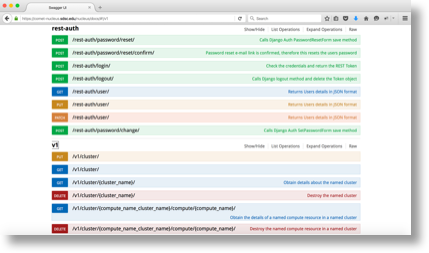
\includegraphics[width=1.0\columnwidth]{images/client/Picture1.png}
    \caption{Rest Interface}
    \label{F:1}
%\end{figure}

%\begin{figure}[htb]
  \centering
    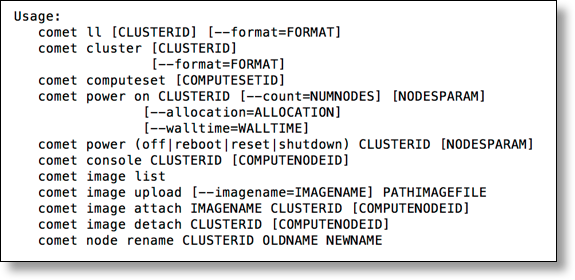
\includegraphics[width=1.0\columnwidth]{images/client/Picture2.png}
    \caption{Commandline }
    \label{F:2}
%\end{figure}

%\begin{figure}[htb]
  \centering
    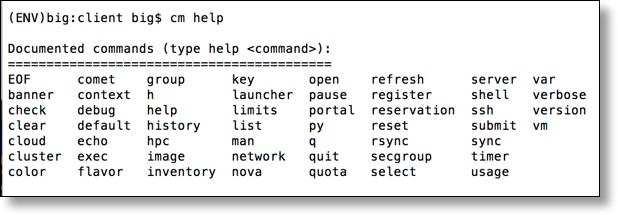
\includegraphics[width=1.0\columnwidth]{images/client/Picture3.png}
    \caption{Command Shell}
    \label{F:3}
%\end{figure}
\end{comment}






\begin{comment}
\begin{figure}[htb]
  \centering
    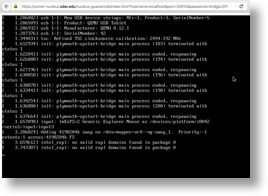
\includegraphics[width=1.0\columnwidth]{images/client/Picture4.png}
    \caption{4}
    \label{F:4}
\end{figure}
\end{comment}

\begin{comment}
%\begin{figure}[htb]
  \centering
    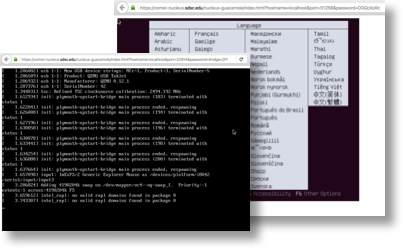
\includegraphics[width=1.0\columnwidth]{images/client/Picture5.png}
    \caption{Console}
    \label{F:5}
\end{figure}
\end{comment}



%%% Local Variables:
%%% mode: latex
%%% TeX-master: t
%%% End:

\section{Results and Usecases} \label{S:results}

We report on some of our use cases while focussing in particular on
the use of virtual machines and virtual clusters, as well as giving an
outlook of selected planned improvements based on lessons learned.

\subsection{Heterogeneous VM Management}

Over the last 2 years we have used Cloudmesh in a number of classes
and research projects to access clouds from a variety of sources. This
includes the management of classes with more than 70 users, but also
the support of individual researchers with the need to conduct
infrastructure experiments. Cloudmesh has been shown to be able to
access Chameleon Cloud, CloudLab, Cybera in Canada, HP cloud, Amazon
WS, Azure. Most recently we also showcased potential access to
Jetstream. One of the interesting benefits of this rich diversity is
that educational efforts can be targeted for a particular platform
while the interface to them for managing virtual machines is the same.
In our experience with classes and potential user this is
an advantage, as when the switch of a single variable (e.g., the
name of the cloud) a VM or VC can be created on
a different infrastructure reducing the load on the original
system. Hence, reliability can be increased without introducing
additional complex and divergent interfaces for the diverse set of
clouds. Future use cases will include class use of {\em Comet\/} VC
for a planned graduate course that can serve up to 140 new
applicants to the newly created data science program at Indiana
University. As we demonstrated with Cloudmesh Client we would also be
able to access other XSEDE resources such as Jetstream and Bridges
once they become available to us and offer programable interfaces that
we can integrate in Cloudmesh.

\subsection{OnDemand Hackathon Support}

In February 2016 SDSC hosted a hackathon \cite{caida} related to the activities of
CAIDA the Center for Applied Internet Data Analysis. ``CAIDA provides macroscopic insights into
Internet infrastructure, behavior, usage, and evolution, fosters a
collaborative environment in which data can be acquired, analyzed, and
(as appropriate) shared, improves the integrity of the field of
Internet science, and informs science, technology, and communications
public policies.''  The hackathons theme was live measurements and
monitoring of the global Internet routing system (BGP). A total of 90
attendees participated in the event representing a mix of Academia,
Industry and Institutions. {\em Comet\/} provided compute resources to
participants, including several virtualized nodes, that were essential
for the success of the event. Over 15,000 SUs were used during 24
hours of activities. The virtualized nodes were especially important
as they allowed CAIDA adminstrators to install a different OS and
application software stack than that which exists on {\em Comet\/}.

\subsection{Open Science Grid}

The Open Science Grid (OSG) \cite{osg} provides an integrated facility
to access compute resources through distributed high throughput
computing for researchers in the US. The resources are contributed by
the community and organized by OSG. Many projects are executed on OSG,
one of which is the Laser Interferometer Gravitational-Wave
Observatory (LIGO). LIGO is ``designed to open the field of
gravitational-wave astrophysics through the direct detection of
gravitational waves predicted by Einstein's General Theory of
Relativity'' \cite{ligo}.

{\em Comet\/} has delivered 700,000 SUs to LIGO via OSG since its
inception. Thus {\em Comet} contributed considerably to both
efforts, OSG and LIGO. In November 2015 OSG began operating a VC on
{\em Comet} and immediately began running calculations related to LIGO. The
integration within OSG has been conducted in two modes to demonstrate
its wide usability (see Figure \ref{F:osg}).

\begin{figure}[htb]
  \centering
    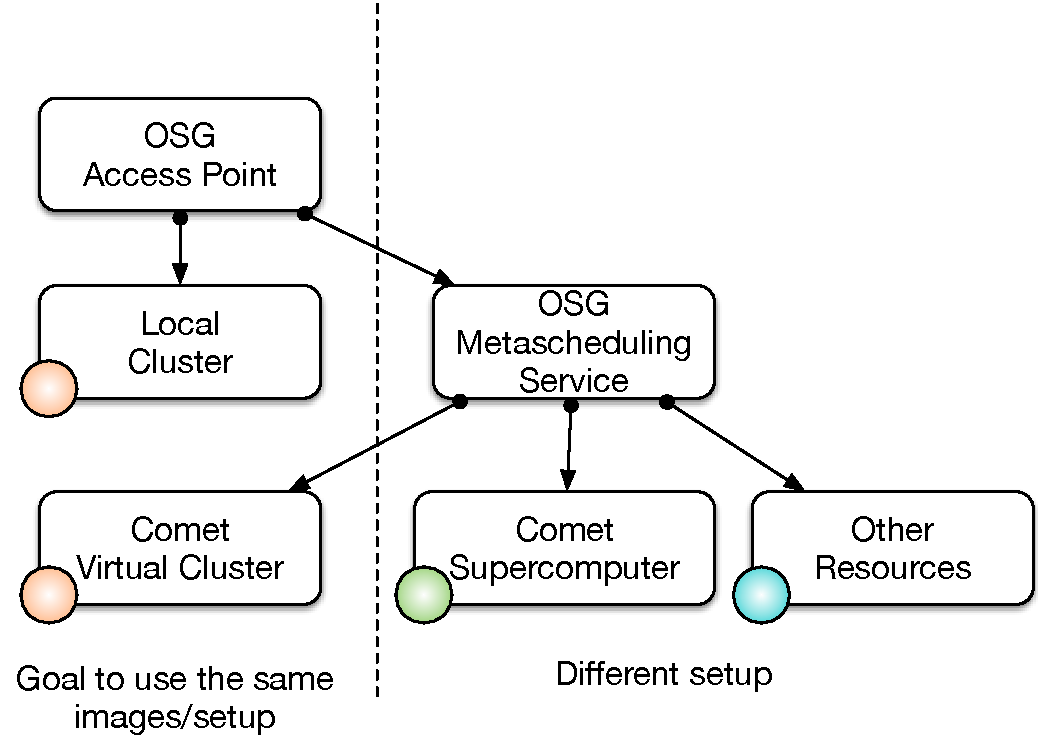
\includegraphics[width=1.0\columnwidth]{images/osg.pdf}
    \caption{Open Science Grid use cases}
    \label{F:osg}
\end{figure}

The first mode is the traditional integration of a supercomputing
allocation while utilizing the batch system and existing specialized
integration of batch job capabilities accessed by the OSG
metascheduler. This mode requires additional layers of abstraction
between the OSG metascheduler and the batch system on the compute
resource. The second one is the integration of a VC
that is based on software used for the operation of the local OSG
cluster and thus shares the same infrastructure requirements in
regards to operating system and other services. Hence no abstraction layer is
needed as a standard OSG system definition and software stack can be
used and run on the VC.  In contrast to other virtualization infrastructures and
efforts we are currently exploring the utilization of MPI jobs within
the VC to make use of the underlying high performance
networking infrastructure accessible from within the OSG VMs. These
VMs already utilize the virtualized InfiniBand HCAs to access storage.



%%% Local Variables:
%%% mode: latex
%%% TeX-master: t
%%% End:


\section{Conclusions} \label{S:conclusion}

We have proven that it is possible to integrate virtual machine
management leveraging an existing HPC batch queuing systems as part of the
operation of a major national scale compute infrastructure. This novel technology solution and
operational model provides the ability to integrate best practices
from both approaches, traditional supercomputing and utilizing
virtual machines to further the long tail of science. Overall
management of such a system is reduced as it
is well integrated in to HPC administrators familiar toolset. This
applies both to the operation of {\em Comet} and the virtual clusters
it hosts.

Additionally, we developed a powerful client interface to {\em Comet}'s
virtualization system.  The Cloudmesh client was developed with the
goal to interface easily and to enable its users to have access
programmatically to {\em Comet} via a Python API, a command shell, a
commandline tool and a prototype portal. Furthermore as new features
become available the client provides an easy mechanism to be updated.

We have utilized the tools and capabilities provided in this paper in a
variety of different scenarios and shown that they are beneficial for
the particular effort. As part of our efforts new use cases, namely
training and development, have emerged.

We will expand upon our current already operational prototypes and
integrate them into a production system that will be available
soon (during Q2 2016). Users that are interested today to explore the virtual modality of
{\em Comet} or Cloudmesh client for comet should contact the authors of the
paper.


\section{Acknowledgments}

Comet is supported by NSF grant: ACI \#1341698 Gateways to Discovery:
Cyberinfrastructure for the Long Tail of Science. 

\bibliographystyle{abbrvurl}
\bibliography{references}


\end{document}
